\documentclass{article}
\usepackage[a4paper, total={6in, 8in}]{geometry}
\usepackage{graphicx}
\usepackage{url}
\usepackage{natbib}
\usepackage{authblk}
\usepackage{todonotes}


\makeatletter
\renewcommand{\maketitle}{\bgroup\setlength{\parindent}{0pt}
	\begin{flushleft}
		
		{\huge\textbf{\@title}}
		
		\bigskip
		
		{\large\textbf{\@author}}
		
		\bigskip
		
		%{\large{Draft current \@date}}
		
	\end{flushleft}\egroup
}
\makeatother


\begin{document}
	% Title
	\title{A Machine-Assisted Systematic Map of Climate Impacts Evidence}
	\author[1,2]{Max Callaghan}
	
	\affil[1]{Mercator Research Institute on Global Commons and Climate Change, Torgauer Straße, 10829 Berlin, Germany}
	\affil[2]{School of Earth and Environment, University of Leeds, Leeds LS2 9JT, United Kingdom}
	\maketitle

	\section{Introduction}
	
	Chapter 18 of working group II's fifth assessment report[ref] presented emerging evidence on the detection and attribution of the impacts of recent changes in climate on natural and human systems. Evidence  collected from hundreds of sources is synthesised in a world map of high-level regional impacts (figure \ref{map}).
	
	This paper aims to use the studies and their labels given in chapter 18 to 
	\begin{itemize}
		\item Develop a query to capture literature on detection and attribution
		\item Develop a machine-learning approach to predict unseen labels and classify unlabelled literature (that which has been published since AR5 or was not included in AR5 chapter 18)
		\item Reproduce an updated, more detailed, more systematic and interactive version of the map produced by IPCC
		\item Point to literature, themes and locations that will help the IPCC to reproduce a similar map in further assessment reports 
	\end{itemize}
	
	
	
	\begin{figure}
		\begin{center}
		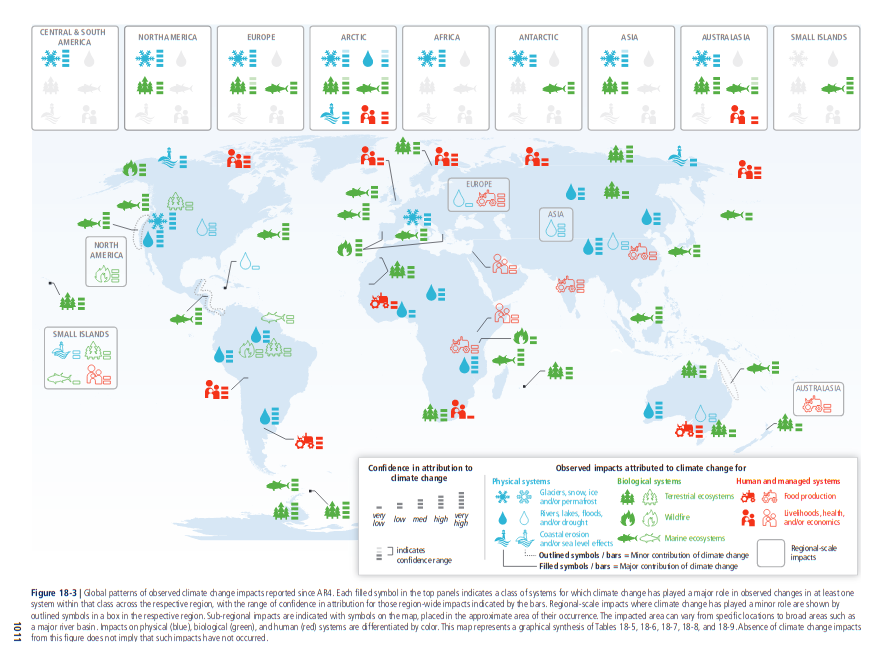
\includegraphics[width=0.7\linewidth]{map_18.png}
		\label{map}
		\end{center}
		\caption{AR5 WGII Chapter 18 synthesis map}
	\end{figure}

	\section{Approach}
	
	[Current to-do list]
	
	\begin{itemize}
		\item Download literature list from WGII tables 18.5-18.9
		\item Develop a query that captures it all
		\item Test query for coverage of other literature, false positives, etc.
		\item Develop coding scheme based on table
		\item Code chapter 18 documents using table
		\item Machine-learning using document classifications
		\begin{itemize}
			\item Test on heldback sample \todo{large enough N? Code some unseen documents?}
			\item Apply to unseen documents
		\end{itemize}
		\item interactive map/database?
	
		
	\end{itemize}
	

	\section{Coding}
	
	\subsection{Table variables}
	
	\textbf{Region:} Africa, Europe, Asia, Australasia, North America, South and Central America, Polar Regions \todo{Is it best to predict having learnt the regions, or to look for place words, or a combination of both?}
	
	\noindent\textbf{System:} Mountains, snow and ice; Rivers, lakes and soil moisture; Terrestrial Ecosystems; Coastal and Marine Ecosystems; Human and Managed Systems
	
	\noindent\textbf{Specific Impact:} Retreat of tropical highland glaciers in East Africa; Increase in rock slope failures in western Alps \ldots	\todo{Intermediate categorisation? Floods, wildfires etc.?}
	
	\noindent\textbf{Confidence in detection:} \textit{Very high, High, Medium, Low}
	
	\noindent\textbf{Role of Climate:} \textit{Major, Minor}
	
	\noindent\textbf{Climate Driver:} Change in Precipitation; Warming; Change in snow cover
	
	\noindent\textbf{Reference behaviour:} No change; Changes due to land use; etc.
	
	\noindent\textbf{Confidence in attribution:} \textit{Very high, High, Medium, Low}
	


		
\end{document}